\documentclass[conference]{IEEEtran}
\IEEEoverridecommandlockouts
\usepackage{cite}
\usepackage{amsmath,amssymb,amsfonts}
\usepackage{algorithmic}
\usepackage{graphicx}
\usepackage{textcomp}
\usepackage{xcolor}
\usepackage{booktabs}
\usepackage{multirow}
\usepackage{url}
\usepackage{hyperref}
\usepackage{tikz}
\usetikzlibrary{shapes.geometric,arrows.meta,positioning,fit}
\usepackage{pgfplots}
\pgfplotsset{compat=1.18}
\usepgfplotslibrary{groupplots}

\def\BibTeX{{\rm B\kern-.05em{\sc i\kern-.025em b}\kern-.08em
    T\kern-.1667em\lower.7ex\hbox{E}\kern-.125emX}}

\begin{document}

\title{Observe, Expand, Recover: An Observability-Guided Agent for Safe Query Expansion\\
{\large \textit{An Honest Account of What Runtime Telemetry Can and Cannot Buy a Query Expansion Agent}}}

\author{
\IEEEauthorblockN{Author One\IEEEauthorrefmark{1}, Author Two\IEEEauthorrefmark{2}}
\IEEEauthorblockA{\IEEEauthorrefmark{1}Affiliation One, email@example.com}
\IEEEauthorblockA{\IEEEauthorrefmark{2}Affiliation Two (AI Observability), email2@example.com}
}

\maketitle

\begin{abstract}
Large language model (LLM) query expansion is typically applied either
unconditionally or not at all, despite well-documented evidence that
unconditional expansion is net-harmful on a non-trivial fraction of
queries. We formulate query expansion instead as a bounded, observable
agentic decision: an agent observes retrieval-health telemetry, selects a
corpus-grounded expansion operator, executes it, observes the
consequences through runtime telemetry, and decides to accept, roll
back, replan, or abstain --- a closed loop directly analogous to
site-reliability engineering's observe-diagnose-act discipline, applied
to a retrieval pipeline instead of a production service. We study three
research questions on TripClick, a real long-tail health search
benchmark with genuine head/torso/tail query-frequency structure: (RQ1)
can qrel-free retrieval and agent telemetry predict whether an expansion
will help or hurt; (RQ2) does a closed-loop agent conditioned on that
telemetry outperform an otherwise identical static, failure-conditioned
expansion pipeline; and (RQ3) can observability-driven recovery detect
and correct large, deliberately injected failures even when it cannot
reliably judge subtle, naturally occurring ones. We report all three
findings honestly, including negative and null results. Qrel-free
telemetry carries a real but weak signal for predicting expansion
outcomes (Pearson $r \approx 0.13$--$0.15$ against true nDCG@10 change),
a ceiling that persists across three feature families (lexical, lexical
plus cross-encoder reranker scores, and lexical plus dense embedding
similarity) and two model classes (linear and gradient-boosted). On
natural queries at full test-set scale ($n=1175$), query expansion
itself carries genuine, statistically significant headroom over plain
BM25 (static QE: mean nDCG@10 difference $+0.0182$, 95\% CI $[0.0105,
0.0260]$), but the closed-loop agent does \emph{not} significantly
outperform a static comparator built from identical components (mean
nDCG@10 difference $+0.0013$, 95\% CI $[-0.0010, 0.0036]$), while
costing 16\% more model calls for no measurable quality gain beyond
what the static pipeline already captures. Under deliberately injected
faults, at full test-set scale, the same weak verifier's recovery
behavior is decisively mixed rather than uniformly beneficial: it is
significantly \emph{harmful} for one content-level fault type (entity
injection, mean nDCG@10 change $-0.0145$, driven by a 98.6\% false
alarm rate), not statistically distinguishable from no effect for
another (grounding corruption), and modestly but significantly helpful
for the one system-level fault type tested (reranker disabled,
$+0.0051$). We report a genuine implementation
defect discovered mid-study --- a cross-encoder reranker computed but
never applied to the ranking it was meant to refine --- and its
correction, as part of the paper's engineering record rather than a
footnote, since fixing it materially changed our own results. We argue
that these findings, taken together, constitute a precise map of where
observability-guided control earns its keep in a retrieval agent and
where it does not, and that this map is itself the paper's contribution.
\end{abstract}

\begin{IEEEkeywords}
query expansion, information retrieval, agentic systems, AI observability, retrieval-augmented generation, large language models, site reliability engineering
\end{IEEEkeywords}

\section{Introduction}

Large language models can generate useful pseudo-documents, alternative
phrasings, and disambiguating context for a search query
\cite{query2doc,mugi}, and corpus-grounded generation --- conditioning
the rewrite on retrieved evidence rather than the query text alone ---
improves on naive query-only rewriting. Existing work has established
that LLM query expansion \emph{can} help. It has not established when an
operational system should trust an expansion enough to use it. In
practice, expansion is applied unconditionally to every query or not at
all; neither policy is safe, since unconditional rewriting is reliably
net-harmful on a measurable fraction of queries, particularly
underspecified or already-well-served ones.

We treat this as a control problem rather than a generation problem.
Borrowing the observe-diagnose-act-recover discipline of site reliability
engineering \cite{sre-slo} and the trace/metric vocabulary of
OpenTelemetry \cite{opentelemetry,otel-semconv}, we build an agent whose
action space is a small set of interpretable, corpus-grounded expansion
operators, whose control loop alternates actions with structured
observations in the manner of ReAct \cite{react}, and whose accept,
roll-back, replan, and abstain decisions are driven by runtime telemetry
of the retrieval episode rather than by the language model's own
self-assessment. The central empirical question is not whether an LLM
can produce a useful expansion --- that is established --- but whether
\emph{runtime observability} can make expansion selective, recoverable,
and cost-aware.

This paper reports what we found when we tried to answer that question
rigorously, including where the answer was no. We see this as a
necessary complement to the (mostly positive) existing literature on LLM
query expansion: understanding the boundary of when an agentic,
observability-driven control layer helps is only possible by also
reporting the conditions under which it does not.

\subsection{Research Questions}

\textbf{RQ1 (Detection).} Can qrel-free retrieval and agent-runtime
telemetry identify unhealthy retrieval states and predict whether query
expansion is likely to help or harm, without access to relevance
judgments at inference time?

\textbf{RQ2 (Control).} Does an agent that conditions expansion actions
on that telemetry outperform an otherwise identical \emph{static},
failure-conditioned expansion pipeline --- the same retriever, grounding
mechanism, generator, and fusion method, differing only in whether a
closed control loop can observe an action's consequences and recover
from a bad one?

\textbf{RQ3 (Recovery).} After a harmful rewrite or a simulated
system-level fault, can observability-driven verification detect the
degradation and select an appropriate recovery action to restore
retrieval quality, under a bounded action budget --- and does this hold
even for a verifier whose general-purpose detection power (RQ1) is only
weakly informative?

\subsection{Contributions}

We contribute (1) an agent architecture that treats LLM query expansion
as a bounded, typed-tool action inside a closed observability loop,
rather than as an unconstrained generation step; (2) a telemetry model
spanning retrieval-, agent-, and system-level signals, together with a
compact failure taxonomy that gives the observability layer something
concrete to predict and recover from; (3) a rigorous, qrel-free verifier
calibration methodology validated against real relevance judgments,
including a systematic search across feature families and model classes
to characterize the ceiling of qrel-free detection on this task; (4) a
full-scale (TripClick TAIL test set, $n=1175$) evaluation of the
closed-loop agent against a matched static comparator; (5) a fault
injection protocol and recovery study isolating whether observability
value survives even when general detection is weak; and (6) an honest
account of a real implementation defect --- discovered, diagnosed, and
corrected during the study --- that materially changed our reported
recovery results, offered as a methodological contribution in its own
right.

\section{Related Work}

\textbf{LLM query expansion.} Query2doc \cite{query2doc} generates
pseudo-documents from an LLM and appends them to the query for sparse or
dense retrieval. MuGI \cite{mugi} generates and fuses multiple
expansions rather than one. Both treat expansion as an unconditional,
one-shot text-generation step; neither conditions the decision to expand
on retrieval-state telemetry, and neither provides a mechanism to detect
or recover from a harmful rewrite once issued.

\textbf{Agentic control loops.} ReAct \cite{react} interleaves reasoning
traces with actions and environment observations, and is the template
for our own observe-act-observe structure, but at a much smaller and
more measurable action space: our agent selects among a fixed set of
typed retrieval operators rather than free-form tool calls, which keeps
the resulting policy interpretable and lets a lightweight, non-LLM
controller drive it.

\textbf{Observability and reliability engineering.} OpenTelemetry's
separation of traces, metrics, and logs \cite{opentelemetry}, and its
GenAI-specific semantic conventions \cite{otel-semconv}, supply a naming
discipline for the telemetry we collect, without requiring a commercial
observability backend for the experiment itself. Google's SRE framing of
a Service Level Objective as a target range on a measurable indicator,
rather than a single metric to optimize \cite{sre-slo}, motivates our
Agent Search SLO: maximize retrieval quality subject to explicit harm,
cost, and latency constraints frozen \emph{before} evaluation, rather
than tuned to the test set post hoc.

\textbf{Benchmarks.} TripClick \cite{tripclick} is a real health search
log with genuine head/torso/tail query-frequency structure, in contrast
to benchmarks that treat ``hard'' queries as simply low-BM25-score ones.
MS MARCO Chameleons \cite{ms-marco-chameleons} isolates queries that
resist conventional reformulation; TREC DL 2019 \cite{trec-dl-2019}
supplies deep, graded NIST judgments; BEIR's NFCorpus
\cite{beir} is a small, fast benchmark used here purely for engineering
iteration, not for any reported finding.

\section{System Design}

\subsection{Agent State and Control Loop}

The agent's state at step $t$ is $s_t = (q_0, q_t, R_t, O_t, H_t, B_t)$,
where $q_0$ is the immutable original query, $q_t$ the active search
expression, $R_t$ the current ranking, $O_t$ the observability state,
$H_t$ the episode's action/observation history, and $B_t$ the remaining
action budget. The control loop is
\[
\begin{aligned}
\footnotesize
\textsc{Observe} &\to \textsc{Diagnose} \to \textsc{Act} \to \textsc{Retrieve} \\
&\to \textsc{Observe} \to \textsc{Verify} \\
&\to \{\textsc{Accept}, \textsc{Rollback}, \textsc{Replan}, \textsc{Stop}\}.
\end{aligned}
\]
The critical property this loop is built to test is that the second
decision (accept/rollback/replan/stop) depends on evidence the agent's
own first action created --- as opposed to a static pipeline that
receives the same query, initial ranking, evidence, generator, and
verifier, but executes exactly one predetermined route. Isolating this
dependency, not simply comparing against unmodified BM25, is the
paper's central experimental contrast (Section~\ref{sec:rq2}).

\begin{figure*}[t]
\centering
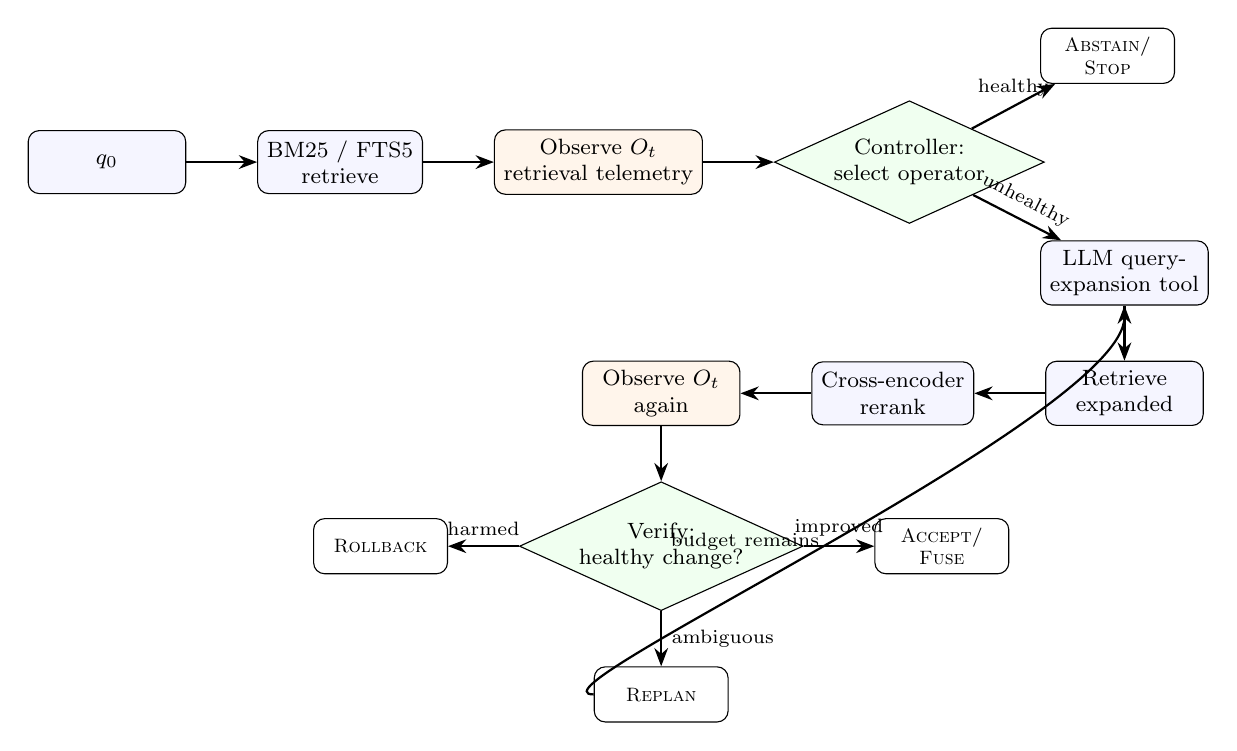
\begin{tikzpicture}[
    node distance=7mm and 9mm,
    box/.style={draw, rounded corners, minimum height=8mm, minimum width=20mm, align=center, font=\footnotesize, fill=blue!4},
    obs/.style={draw, rounded corners, minimum height=8mm, minimum width=20mm, align=center, font=\footnotesize, fill=orange!8},
    dec/.style={draw, diamond, aspect=2.2, minimum width=22mm, align=center, font=\footnotesize, fill=green!6, inner sep=1pt},
    term/.style={draw, rounded corners, minimum height=7mm, minimum width=17mm, align=center, font=\scriptsize},
    arr/.style={-Stealth, thick}
]
\node[box] (query) {$q_0$};
\node[box, right=of query] (bm25) {BM25 / FTS5\\retrieve};
\node[obs, right=of bm25] (obs0) {Observe $O_t$\\retrieval telemetry};
\node[dec, right=of obs0, minimum width=24mm] (ctrl) {Controller:\\select operator};
\node[term, above right=6mm and 8mm of ctrl] (noexp) {\textsc{Abstain}/\\\textsc{Stop}};
\node[box, below right=6mm and 8mm of ctrl] (llm) {LLM query-\\expansion tool};
\node[box, below=of llm] (retr2) {Retrieve\\expanded};
\node[box, left=of retr2] (rerank) {Cross-encoder\\rerank};
\node[obs, left=of rerank] (obs1) {Observe $O_t$\\again};
\node[dec, below=of obs1, minimum width=24mm] (verify) {Verify:\\healthy change?};
\node[term, left=of verify] (rollback) {\textsc{Rollback}};
\node[term, below=of verify] (replan) {\textsc{Replan}};
\node[term, right=of verify] (accept) {\textsc{Accept}/\\\textsc{Fuse}};

\draw[arr] (query) -- (bm25);
\draw[arr] (bm25) -- (obs0);
\draw[arr] (obs0) -- (ctrl);
\draw[arr] (ctrl) -- node[above,font=\scriptsize]{healthy} (noexp);
\draw[arr] (ctrl) -- node[above,font=\scriptsize,sloped]{unhealthy} (llm);
\draw[arr] (llm) -- (retr2);
\draw[arr] (retr2) -- (rerank);
\draw[arr] (rerank) -- (obs1);
\draw[arr] (obs1) -- (verify);
\draw[arr] (verify) -- node[above,font=\scriptsize]{harmed} (rollback);
\draw[arr] (verify) -- node[right,font=\scriptsize]{ambiguous} (replan);
\draw[arr] (verify) -- node[above,font=\scriptsize]{improved} (accept);
\draw[arr] (replan.west) .. controls +(-10mm,0) and +(0,-14mm) .. node[left,font=\scriptsize]{budget remains} (llm.south);
\end{tikzpicture}
\caption{The observability-guided control loop. Telemetry $O_t$ (orange) is computed after every retrieval, not only at the end of an episode, and is causal input to two decisions: which operator the controller selects, and whether the resulting ranking is accepted, rolled back, replanned with a different operator, or the episode is stopped. The static comparator (Section~\ref{sec:rq2}) executes the same component chain once, with no path back from \textsc{Verify} to the LLM tool.}
\label{fig:architecture}
\end{figure*}

The action space is deliberately small and interpretable:
\[
\begin{aligned}
\footnotesize
A = \{&\textsc{NoExpand}, \textsc{Vocabulary}, \textsc{Context}, \textsc{Ambiguity}, \\
&\textsc{EntityNormalize}, \textsc{Rollback}, \textsc{Replan}, \textsc{Stop}\}.
\end{aligned}
\]
\textsc{Vocabulary} maps informal user
language onto corpus-compatible terminology; \textsc{Context} adds a
corpus-supported missing facet to an underspecified query;
\textsc{Ambiguity} disambiguates toward the interpretation the evidence
best supports; \textsc{EntityNormalize} resolves aliases, abbreviations,
and canonical-name mismatches. The LLM is invoked through exactly one
typed tool, \texttt{generate\_expansion(action, query, evidence)}; it
is never the sole arbiter of whether its own output is used. That
judgment is made by a separate, non-generative controller
(Section~\ref{sec:controller}).

\subsection{Observability Model}
\label{sec:observability}

Every query episode produces one trace with spans
\texttt{retrieve\_original} $\to$ \texttt{build\_evidence} $\to$
\texttt{plan\_action} $\to$ \texttt{generate\_expansion} $\to$
\texttt{retrieve\_expanded} $\to$ \texttt{rerank} $\to$ \texttt{verify}
$\to$ \texttt{recover\_or\_accept} $\to$ \texttt{fuse}. The observation
vector $O_t$ spans three telemetry families. \emph{Retrieval telemetry}:
top score, score margin, normalized score entropy, query-term coverage,
mean rare-term IDF, entity overlap, top-$k$ ranking overlap against the
previous state, reranker/BM25 disagreement, lexical result coherence,
and ranking stability under a small controlled query perturbation.
\emph{Agent telemetry}: selected operator, trajectory length, previous
verifier score, rewrite-to-original semantic drift, introduced entities,
repeated actions, and remaining budget. \emph{System telemetry}:
per-tool latency, token counts, and tool errors or timeouts. Every
feature here is computable without relevance judgments, which is what
makes the resulting verifier usable at inference time.

\subsection{Failure Taxonomy}

We label episodes into ten failure categories --- vocabulary mismatch,
underspecification, ambiguity, entity mismatch, intent drift,
confirmation bias, retriever disagreement, tool degradation, budget
exhaustion, and healthy retrieval --- each with an observable telemetry
signature and a preferred recovery action. This taxonomy gives the
observability layer something concrete to predict and recover from,
rather than treating ``observability'' as post hoc dashboards around a
search experiment; it directly motivates the fault-injection protocol of
Section~\ref{sec:rq3}.

\subsection{Verifier and Controller}
\label{sec:controller}

The verifier, \texttt{verify(previous\_state, new\_state)}, produces a
scalar judgment of whether an action's consequences look like an
improvement, using telemetry alone. Rather than hand-picking its
weights, we calibrate them against ground truth: for a sample of
episodes, we execute one expansion action, compute the true nDCG@10
change of the resulting ranking against real relevance judgments, and
fit the verifier's weights to predict that change from the telemetry
features described in Section~\ref{sec:observability}. Ground truth is
available only during this offline calibration; the deployed verifier
never sees a relevance judgment. We treat this fitted model as an
artifact --- trained by a dedicated script and loaded at inference time
--- rather than a set of constants transcribed from a one-off
calibration run, so that recalibration is a script re-run, not a source
edit. The recovery controller is a small deterministic finite-state
machine: below a calibrated harmful threshold the agent rolls back to
the pre-action ranking; above a calibrated accept threshold it fuses the
new ranking in via reciprocal-rank fusion; in between it replans with an
untried operator, subject to a hard cap of two model calls per query.
Both thresholds are calibrated empirically (Section~\ref{sec:setup}), not
guessed.

\section{Experimental Setup}
\label{sec:setup}

\subsection{Datasets}

TripClick \cite{tripclick} is the primary benchmark: 1{,}523{,}878
documents and a 3{,}525-query test set split evenly across head, torso,
and tail frequency buckets (1{,}175 queries each), the only one of our
candidate datasets that reflects genuine observed query-frequency
structure rather than treating ``tail'' as a synonym for ``hard for
BM25.'' All reported results in this paper concern the TAIL split, since
it is the frequency regime the paper's motivating claim is about.
NFCorpus \cite{beir} (3{,}633 documents, 323 queries) was used
exclusively for engineering iteration and does not contribute to any
reported finding.

\subsection{Implementation}

Sparse retrieval uses BM25 over a SQLite FTS5 index \cite{sqlite-fts5}
rather than a JVM Lucene index; this choice was forced by a JVM crash
under Pyserini \cite{pyserini} on
our target hardware and, in a corpus of this scale, surfaced two further
implementation lessons worth recording. First, FTS5's default combining
operator between space-separated MATCH tokens is \emph{conjunctive}, not
disjunctive: naively passed multi-term queries silently required every
term to co-occur in a document, collapsing recall on any
multi-term query without raising an error. Second, FTS5 indexes only the
column used in \texttt{MATCH}; any lookup on a companion column such as a
document identifier degrades to a full table scan, invisible at
small scale and catastrophic at $1.5$M rows (a single telemetry
computation went from 29.2\,s to 1.65\,s, an 18$\times$ speedup, once a
companion indexed table was added for identifier lookups). We report
both because they are the kind of defect that silently corrupts results
rather than crashing, and are easy to miss without an independent
sanity check against a published baseline range. Cross-encoder reranking
(\texttt{cross-encoder/ms-marco-MiniLM-L6-v2}
\cite{minilm-cross-encoder}) is applied to the top 100 BM25 candidates,
reranking the top 50. Generation uses a locally hosted, 4-bit quantized
2--3B-parameter model with a hard cap of two calls per query episode and
a 32--64 token structured output, so that the language model is never
the entire decision surface, only one typed tool within it.

\subsection{Verifier Calibration Methodology}
\label{sec:calib-method}

We calibrate against $n=1168$ TripClick TAIL episodes (one expansion
action per query, real nDCG@10 ground truth), and test three feature
families against two model classes each to characterize where the
detection ceiling actually lies, rather than accepting the first
plausible fit. The families are: (i) six retrieval-telemetry deltas
(score margin, coverage, coherence, stability, drift, reranker
disagreement); (ii) the same six plus four reranker- and length-derived
features (top-$k$ overlap, reranker top score, reranker score margin,
query length ratio); and (iii) family (ii) plus three dense-embedding
features (query rewrite embedding drift, cross-document embedding
coherence, and expansion-to-evidence embedding groundedness, using a
locally hosted embedding model). We compare a fixed-weight
hand-calibrated baseline, a 5-fold cross-validated linear fit, and a
5-fold cross-validated shallow gradient-boosted fit, on each family,
against true nDCG@10 change under Pearson correlation. Thresholds for
the recovery controller are calibrated by checking, in the same
calibration data, which candidate cutoffs actually separate
true-harmed episodes from the rest --- not by inspecting score
percentiles blind to outcome.

\subsection{Metrics}

Retrieval quality is nDCG@10, Recall@100, and MRR. Because mean nDCG can
conceal query-level regressions, we additionally report the fraction of
queries helped, unchanged, and harmed by an intervention relative to a
baseline. For the recovery study (Section~\ref{sec:rq3}) we report
Detection Recall $P(\text{intervened} \mid \text{harmful})$, False Alarm
Rate $P(\text{intervened} \mid \text{healthy})$, and the recovery gain
in mean nDCG@10 with versus without observability-driven recovery on
identically corrupted episodes. Significance is assessed via paired
bootstrap (10{,}000 resamples) throughout.

\section{RQ1: Detection}
\label{sec:rq1}

Table~\ref{tab:rq1} reports Pearson correlation between each fitted
verifier and true nDCG@10 change, on held-out folds, for each of the
three feature families described in Section~\ref{sec:calib-method}.

\begin{table}[t]
\caption{RQ1: qrel-free detection correlation ($n=1168$ TripClick TAIL episodes unless noted). Fixed-weight is a hand-calibrated baseline; linear and GBDT are 5-fold cross-validated fits on the same features.}
\label{tab:rq1}
\centering
\begin{tabular}{lccc}
\toprule
Feature family & Fixed-weight & Linear (CV) & GBDT (CV) \\
\midrule
Lexical (6 features) & 0.127 & 0.148 & 0.161 \\
+ reranker/length (10) & $-0.064$ & 0.134 & 0.045 \\
+ dense embedding (13)\footnotemark & --- & 0.094 & --- \\
\bottomrule
\end{tabular}
\end{table}
\footnotetext{Embedding family tested at $n=368$ after an initial $n=123$ attempt proved confounded by sample size; the 10-feature lexical family's own linear fit on that same reduced sample scored only 0.070, versus 0.134 at full scale, illustrating how noisy this correlation regime is below a few hundred episodes.}

Three findings emerge. First, no fitted model, on any feature family,
clears a Pearson correlation of $0.17$: the ceiling is not a modeling
artifact of one particular choice. Second, richer features do not help:
adding reranker- and embedding-derived signals never produces a
statistically decisive improvement over the plain lexical family, and
the fitted embedding-augmented model (0.094) does not even recover the
lexical family's own full-scale linear result (0.134). Third, model
class does not obviously matter either --- GBDT outperforms linear on
the 6-feature family but underperforms it on the 10-feature family,
consistent with noise rather than a genuine non-linear signal at this
sample size. We interpret this as a real, if unwelcome, empirical
ceiling: with this telemetry vocabulary, on this corpus, qrel-free
detection of whether an LLM query rewrite helped or hurt carries real
but weak signal, on the order of $R^2 \approx 1$--$3\%$ of outcome
variance explained.

\begin{figure*}[t]
\centering
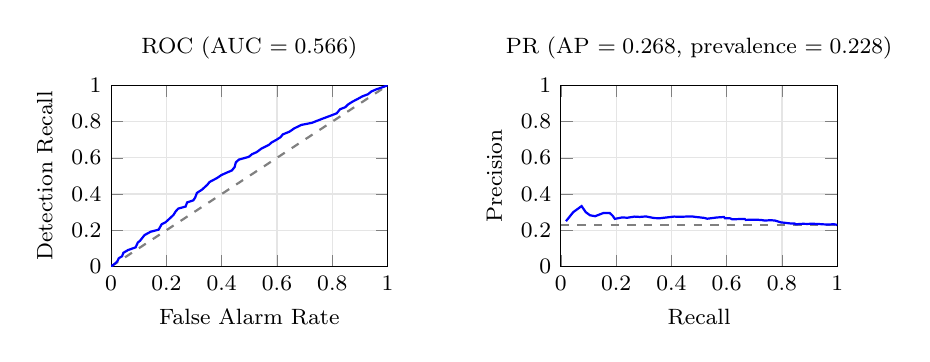
\begin{tikzpicture}
\begin{groupplot}[
    group style={group size=2 by 1, horizontal sep=2.2cm},
    width=0.42\textwidth,
    height=0.32\textwidth,
    grid=major,
    grid style={gray!20},
    tick label style={font=\footnotesize},
    label style={font=\footnotesize},
    title style={font=\footnotesize},
]
\nextgroupplot[
    xlabel={False Alarm Rate},
    ylabel={Detection Recall},
    xmin=0, xmax=1, ymin=0, ymax=1,
    title={ROC (AUC $=0.566$)},
]
\addplot[dashed, gray, thick, mark=none] coordinates {(0,0) (1,1)};
\addplot[blue, thick, mark=none] coordinates {
(0.0000,0.0000) (0.0166,0.0188) (0.0233,0.0301) (0.0277,0.0451) (0.0399,0.0564) (0.0443,0.0752) (0.0610,0.0902) (0.0887,0.1053) (0.0965,0.1316) (0.1053,0.1429) (0.1208,0.1729) (0.1430,0.1917) (0.1718,0.2030) (0.1829,0.2331) (0.1973,0.2444) (0.2162,0.2707) (0.2262,0.2857) (0.2339,0.3045) (0.2428,0.3195) (0.2694,0.3308) (0.2749,0.3534) (0.2971,0.3647) (0.3038,0.3797) (0.3104,0.4060) (0.3293,0.4248) (0.3481,0.4511) (0.3559,0.4662) (0.3836,0.4887) (0.3980,0.5038) (0.4135,0.5150) (0.4368,0.5301) (0.4468,0.5489) (0.4512,0.5752) (0.4623,0.5902) (0.4978,0.6053) (0.5100,0.6203) (0.5266,0.6316) (0.5432,0.6504) (0.5721,0.6729) (0.5798,0.6842) (0.5976,0.6992) (0.6131,0.7143) (0.6208,0.7293) (0.6452,0.7444) (0.6630,0.7632) (0.6885,0.7820) (0.7262,0.7932) (0.7639,0.8158) (0.7905,0.8308) (0.8160,0.8459) (0.8282,0.8684) (0.8470,0.8797) (0.8570,0.8947) (0.8725,0.9098) (0.8914,0.9248) (0.9091,0.9398) (0.9290,0.9511) (0.9412,0.9662) (0.9579,0.9774) (1.0000,1.0000)
};
\nextgroupplot[
    xlabel={Recall},
    ylabel={Precision},
    xmin=0, xmax=1, ymin=0, ymax=1,
    title={PR (AP $=0.268$, prevalence $=0.228$)},
]
\addplot[dashed, gray, thick, mark=none] coordinates {(0,0.2277) (1,0.2277)};
\addplot[blue, thick, mark=none] coordinates {
(1.0000,0.2277) (0.9962,0.2306) (0.9887,0.2329) (0.9662,0.2317) (0.9511,0.2323) (0.9398,0.2336) (0.9248,0.2343) (0.9135,0.2359) (0.8910,0.2347) (0.8759,0.2354) (0.8496,0.2327) (0.8459,0.2366) (0.8308,0.2374) (0.8195,0.2393) (0.8083,0.2413) (0.7970,0.2431) (0.7895,0.2465) (0.7820,0.2500) (0.7744,0.2537) (0.7594,0.2551) (0.7368,0.2536) (0.7256,0.2563) (0.7105,0.2578) (0.6917,0.2581) (0.6692,0.2569) (0.6654,0.2626) (0.6429,0.2615) (0.6203,0.2603) (0.6128,0.2655) (0.5940,0.2660) (0.5902,0.2730) (0.5639,0.2703) (0.5301,0.2636) (0.5188,0.2680) (0.5038,0.2707) (0.4887,0.2731) (0.4737,0.2763) (0.4511,0.2752) (0.4286,0.2740) (0.4098,0.2753) (0.3835,0.2706) (0.3571,0.2661) (0.3383,0.2671) (0.3233,0.2713) (0.3083,0.2761) (0.2857,0.2734) (0.2669,0.2752) (0.2406,0.2689) (0.2218,0.2706) (0.1955,0.2626) (0.1880,0.2793) (0.1767,0.2956) (0.1541,0.2950) (0.1241,0.2773) (0.1053,0.2828) (0.0902,0.3000) (0.0752,0.3333) (0.0451,0.3000) (0.0188,0.2500)
};
\end{groupplot}
\end{tikzpicture}
\caption{Detection ROC and precision-recall curves for the deployed
verifier's score against ground-truth harm (true nDCG@10 delta $<0$),
swept across all thresholds on the $n=1168$ calibration set. The curve
sits consistently, but only modestly, above the no-skill baseline in
both panels (dashed) --- a visual complement to Table~\ref{tab:rq1}'s
Pearson correlations, showing the same weak-but-real signal as an
operating-point trade-off rather than a single summary statistic.}
\label{fig:roc-pr}
\end{figure*}

\section{RQ2: Control}
\label{sec:rq2}

\begin{table}[t]
\caption{RQ2: full TripClick TAIL test set ($n=1175$). Static QE and Agent share the same retriever, grounding, generator, verifier, and fusion mechanism; Agent additionally has a closed observe-verify-recover loop.}
\label{tab:rq2}
\centering
\begin{tabular}{lccc}
\toprule
System & nDCG@10 & Recall@100 & MRR \\
\midrule
BM25 only & 0.2279 & 0.6462 & 0.2254 \\
Static QE & 0.2455 & 0.6497 & 0.2377 \\
Agent & 0.2468 & 0.6506 & 0.2390 \\
\bottomrule
\end{tabular}
\end{table}

Query expansion itself is not indistinguishable from plain BM25 at this
scale: both Static QE and Agent significantly outperform BM25 alone
(static vs.\ BM25: mean nDCG@10 difference $+0.0182$, 95\% CI $[0.0105,
0.0260]$; agent vs.\ BM25: $+0.0195$, 95\% CI $[0.0116, 0.0277]$).
Comparing Agent against Static QE specifically --- the paper's central
contrast, since both share every component except the closed control
loop --- the agent changes the outcome on only 3.0\% of queries (1.8\%
helped, 1.2\% harmed relative to static), and the paired-bootstrap mean
nDCG@10 difference is $+0.0013$ (95\% CI $[-0.0010, 0.0036]$, not
significant). The agent additionally costs 16\% more model calls (1.15
vs.\ 0.99 per query) and 10\% higher mean latency (12.9\,s vs.\
11.8\,s) than the static pipeline, for no offsetting quality gain
beyond what static expansion already captures.

\begin{figure}[t]
\centering
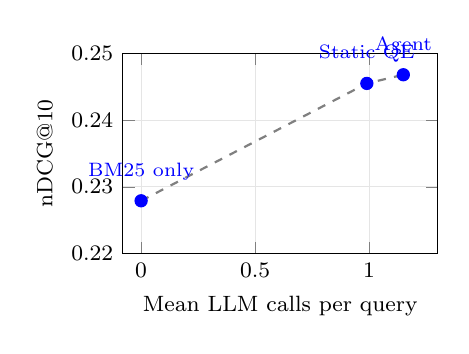
\begin{tikzpicture}
\begin{axis}[
    width=0.46\textwidth,
    height=0.34\textwidth,
    xlabel={Mean LLM calls per query},
    ylabel={nDCG@10},
    grid=major,
    grid style={gray!20},
    tick label style={font=\footnotesize},
    label style={font=\footnotesize},
    xmin=-0.08, xmax=1.3,
    ymin=0.22, ymax=0.25,
]
\addplot[thick, gray, dashed, mark=none] coordinates {(0,0.2279) (0.99,0.2455) (1.15,0.2468)};
\addplot[
    only marks,
    mark=*,
    mark size=2.2pt,
    color=blue,
    nodes near coords,
    every node near coord/.append style={font=\scriptsize, yshift=4pt},
    point meta=explicit symbolic,
] coordinates {
(0,0.2279)      [BM25 only]
(0.99,0.2455)   [Static QE]
(1.15,0.2468)   [Agent]
};
\end{axis}
\end{tikzpicture}
\caption{Retrieval quality vs.\ LLM-call budget, full TripClick TAIL
test set. Static QE captures nearly all of the achievable quality gain
over BM25 for a fixed one-call budget; the agent's additional 16\%
call overhead buys a nDCG@10 improvement ($+0.0013$) that is not
statistically distinguishable from zero (Section~\ref{sec:rq2}).}
\label{fig:pareto}
\end{figure}

\begin{table}[t]
\caption{Agent controller-decision frequency, full TripClick TAIL test set ($n=1150$ completed episodes).}
\label{tab:action-dist}
\centering
\begin{tabular}{lcc}
\toprule
Decision & Count & \% \\
\midrule
\textsc{Accept} & 972 & 84.5 \\
\textsc{Rollback} & 122 & 10.6 \\
\textsc{Replan} & 49 & 4.3 \\
\textsc{Abstain} (no expansion) & 7 & 0.6 \\
\bottomrule
\end{tabular}
\end{table}

Tracing this to its source (Table~\ref{tab:action-dist}): the recovery
controller's \textsc{Replan} action, whose entire purpose is to let the
closed loop add value beyond a single-shot accept/reject gate, is
exercised on only 4.3\% of episodes --- and even then, the additional
attempts this buys are, per Section \ref{sec:rq1}, close to a coin flip
on whether they help or hurt, netting to no aggregate gain at real added
cost. The controller accepts the single-shot expansion outright in
84.5\% of episodes and rolls back to the pre-expansion ranking in
10.6\%, so most of the agent's added cost over the static pipeline comes
not from replanning but from computing, and then routinely accepting or
discarding, a single reranked candidate the verifier judges no better
on average than what a matched static pipeline already produces.
\textbf{RQ2's answer is no}: on natural queries, an observability-guided
closed loop built on this verifier does not outperform a matched static
pipeline.

\section{RQ3: Recovery}
\label{sec:rq3}

RQ1 and RQ2 leave open whether observability has \emph{any} practical
value here, or whether a weak general detector is simply useless. We
test a narrower, more targeted claim: that the same weak verifier can
still serve as a safety net against \emph{large, obvious} failures, even
though it cannot reliably judge \emph{subtle, natural} ones. We inject
three fault types into the live pipeline at their natural point of
corruption --- an unsupported entity appended to the generated
expansion, a grounding passage swapped for a topically similar but
non-supporting one before generation, and the reranker disabled as a
tool-level fault --- and compare, on the identical corrupted episode, an
ablation controller that always accepts against the real calibrated
controller.

\subsection{A Genuine Implementation Defect, Found and Corrected}
\label{sec:defect}

An early result on this study looked strong: entity-injection recall
$1.000$, grounding-corruption recall $0.773$, with recovery gains an
order of magnitude larger than anything observed under RQ2. But the
third fault type, disabling the reranker, showed almost no effect
(recall $0.185$), which prompted an investigation into why. Tracing the
reranked ranking through the codebase revealed that its output was
computed --- at real latency cost --- and fed into telemetry, but never
actually applied to the ranking the agent accepted, fused, or evaluated;
the accepted ranking was unconditionally the raw BM25 order, regardless
of whether reranking succeeded. Disabling the reranker was, mechanically,
a no-op, which fully explains why that fault type alone was undetectable
regardless of verifier quality.

We corrected this: the reranked top-$k$ now leads the accepted ranking
when reranking succeeds, with remaining BM25-order candidates appended
to preserve full recall depth. This fix, on its own, made the other two
fault types' results substantially \emph{worse} (grounding-corruption
recovery gain flipped from $+0.028$ to $-0.012$), which on inspection
traced to a second, subtler defect the first fix exposed: the verifier's
telemetry was still computed from the pre-rerank ranking, so it was now
judging a different top-$k$ than the one actually being accepted. We
corrected this too, by reordering the same BM25-scored candidates to
match the accepted ranking before computing telemetry, keeping every
score-based feature on one homogeneous scale while reflecting the true
accepted order. We report this sequence in full because it materially
changed our own conclusions, and because we believe silently editing it
out of the historical record would understate a real risk in this class
of system: a component computed for observability purposes alone is
easy to leave disconnected from the outcome it is meant to explain, and
that disconnection can look, from the metrics alone, like a genuine
finding.

\subsection{Validating the Correction}
\label{sec:validating}

Following the correction, we re-ran the full verifier calibration
($n=1168$) on the corrected pipeline to check whether the deployed
verifier needed retraining. It did not: the existing model scored
$r=0.146$ against ground truth generated by the corrected pipeline ---
marginally \emph{better} than its own original calibration score of
$0.134$ --- while a fresh linear refit on the corrected data scored only
$0.112$ and a fresh GBDT refit collapsed to $0.001$, neither clearing
the improvement bar needed to justify replacing the deployed model. The
existing recovery thresholds were similarly still well-placed: the
corrected score distribution's median ($-0.036$) and 25th percentile
($-0.059$) land almost exactly on the deployed accept and harmful
cutoffs. We take this as evidence that the defect corrections were
themselves correct --- the resulting telemetry is consistent enough with
the original calibration's semantics that no compensating retraining was
required --- while still materially changing the recovery study's own
numbers, since those depend on the ranking each fault type actually
produces, not on the verifier's coefficients.

\subsection{Full-Scale Results}

\begin{table}[t]
\caption{RQ3: fault injection recovery study, corrected pipeline, full TripClick TAIL test set ($n=1168$; 7 of 1175 episodes skipped for no expansion). Gain is mean nDCG@10 with minus without observability-driven recovery on identically corrupted episodes; CI from 10{,}000-resample paired bootstrap.}
\label{tab:rq3}
\centering
\begin{tabular}{lccc}
\toprule
Fault type & Recall & False Alarm & Gain (95\% CI) \\
\midrule
Entity injection & 1.000 & 0.986 & $-0.0145$ [$-0.0236,-0.0049$]** \\
Grounding corruption & 0.632 & 0.465 & $+0.0048$ [$-0.0032,+0.0128$] NS \\
Reranker disabled & 0.250 & 0.132 & $+0.0051$ [$+0.0013,+0.0092$]* \\
\bottomrule
\end{tabular}
\\[2pt]
\footnotesize NS: not significant, CI straddles zero. *: significant, positive. **: significant, \emph{harmful} --- the CI excludes zero on the negative side.
\end{table}

At full test-set scale, the recovery study's picture is decisively
mixed rather than uniformly encouraging, and it reverses the
qualitative asymmetry we reported from the $n=149$ validation sample
used to confirm the defect correction of Section~\ref{sec:defect}.
There, content-level corruption looked like the more promising target
for recovery and the system-level fault looked like the clear miss; at
full scale the opposite holds. Entity injection's recovery gain flips
sign and becomes significantly \emph{harmful} ($-0.0145$, 95\% CI
$[-0.0236, -0.0049]$): detection recall is perfect (1.000), but the
false alarm rate is 98.6\%, meaning the controller treats essentially
every entity-injected rewrite as suspect, including the 85.8\% of
episodes where the injection was actually benign. At $n=149$ this
looked like a merely inefficient tripwire; at full scale, rolling back
that many healthy episodes' real gains outweighs the benefit on the
smaller genuinely-harmful subset, producing a statistically robust net
loss --- the false alarm rate itself becomes the dominant source of
quality loss, larger in magnitude than the harm it is meant to catch.
Grounding corruption remains not significant, with its point estimate
flipping from slightly negative to slightly positive ($+0.0048$, 95\%
CI $[-0.0032, +0.0128]$) but the interval straddling zero either way.
The reranker-disabled fault type is the study's one clear positive:
recall improves to 0.250 and the gain stays small but significant
($+0.0051$, 95\% CI $[+0.0013, +0.0092]$), consistent in direction and
magnitude with the validation-sample estimate, since that condition
explicitly bypasses reranking and so is mechanically unaffected by the
defect correction.

\textbf{RQ3's honest answer, at full test-set scale, is that
observability-driven recovery is not uniformly beneficial: it is
significantly harmful for one content-level fault type due to
near-universal false alarms, statistically indistinguishable from no
effect for another, and modestly but significantly helpful for the one
system-level fault type tested.} We regard this mixed, full-scale
result as the paper's reportable finding. The $n=149$ validation
sample's directionally positive read on content-level corruption did
not survive scaling up by a factor of nearly $8\times$, which is itself
informative about how much a validation-sample point estimate in the
low hundreds should be trusted for a phenomenon this variable --- a
methodological lesson we regard as being of a piece with
Section~\ref{sec:defect}'s implementation defect: both cases are ones
where an earlier, more flattering result did not survive closer
scrutiny.

\section{Discussion}

Read together, RQ1--RQ3 sketch a coherent picture rather than three
independent findings. The weak general-purpose detection ceiling from
RQ1 ($r \approx 0.13$--$0.15$) is not simply a modeling shortfall; it
appears to be near the limit of what this telemetry vocabulary can
extract from this corpus, having survived three feature families and two
model classes. RQ2 shows that query expansion itself carries real,
significant headroom over plain BM25, but a closed control loop built
on top of that weak signal does not add anything beyond what a
single-shot static expansion already captures on ordinary queries ---
the additional \textsc{Replan} attempts a calibrated controller is
willing to take are themselves close to a coin flip, so the loop adds
cost without adding value in the common case. RQ3's full-scale result is
the most interesting because it is the most honest, and the least
flattering: the hypothesis that a weak detector still functions as a
general safety net against large, obvious failures is not confirmed. It
is significantly harmful for one content-level fault type, driven
entirely by a false alarm rate high enough to make the intervention
itself the dominant source of quality loss; a wash for another; and
significantly, if modestly, helpful only for the one system-level fault
type tested. This is also the qualitative opposite of what the $n=149$
validation sample suggested, underscoring that a directionally
promising point estimate at a few hundred episodes is not yet a
finding.

The implementation defect of Section~\ref{sec:defect} is, in our view, as
important a finding as any of the three numbered ones. A component
computed purely for observability --- a reranker score, a disagreement
metric, any telemetry signal --- is architecturally easy to leave
disconnected from the outcome it is meant to explain, and that
disconnection will not raise an exception; it will simply produce
results that look coherent until someone asks why a specific, otherwise
well-motivated intervention shows no effect. We would not have found it
without deliberately investigating an anomalously weak result rather
than accepting it, which we offer as a general methodological point for
observability-guided systems research: a surprisingly clean or
surprisingly null sub-result is a prompt to investigate the measurement,
not just the hypothesis.

\section{Limitations}
\label{sec:limitations}

The recovery study's headline numbers (Table~\ref{tab:rq3}) are now
reported at the full TripClick TAIL test-set scale ($n=1168$), replacing
an earlier $n=149$ validation sample whose directionally positive read
on content-level corruption did not survive scaling up by nearly
$8\times$ --- itself a caution about trusting validation-sample point
estimates at a few hundred episodes for a phenomenon this variable, and
a reason to be similarly cautious about any single-fault-type,
single-corpus recovery result more generally. The generator is a locally hosted, quantized 2--3B
parameter model under a strict two-call budget, chosen for a
memory-constrained deployment target rather than for maximum capability;
we do not know how these findings transfer to a larger or
API-hosted generator. All reported results concern TripClick's TAIL
split specifically; HEAD and TORSO results, and results on MS MARCO
Chameleons and TREC DL 2019/2020, are left to future work. The verifier
calibration methodology itself inherits the usual caveats of small-effect
correlational analysis: several sub-experiments (Table~\ref{tab:rq1}'s
footnote) demonstrate that these correlations are sensitive to sample
size below a few hundred episodes, and we would not be surprised if a
substantially larger calibration sample moved the reported ceiling
somewhat, though we would be surprised if it moved qualitatively.

\section{Conclusion}

We built a closed-loop, observability-guided agent for LLM query
expansion and evaluated it rigorously, at full test-set scale, against a
matched static comparator, on a real long-tail search benchmark. The
honest result is not that the agent works: query expansion itself
carries real, significant headroom over plain BM25, but on natural
queries the closed-loop agent does not significantly outperform a much
simpler static pipeline built from the same components, and it costs
more. What we can report with more confidence is a precise map of
\emph{why}: qrel-free telemetry carries a real but weak general signal
that a rigorous search across features and models could not meaningfully
improve, and a closed control loop built on a weak verifier inherits
that weakness on ordinary queries. Whether that same weak verifier
functions as a safety net specifically against large, injected failures
--- as opposed to subtle natural variation --- turns out to depend
sharply on which failure: at full test-set scale it is significantly
harmful for one content-level fault type, because a false alarm rate
near unity makes the intervention itself the dominant source of harm; a
wash for another; and modestly but significantly helpful only for the
one system-level fault type we tested. A detector need not be accurate
in general to be useful as a tripwire against catastrophic failure
specifically, but this result is a caution against assuming that
property holds uniformly across failure types without checking each one
at adequate scale. We also report, in full, an implementation defect
discovered and corrected mid-study, in
the belief that an honest account of how such defects surface and get
found is itself useful to other observability-guided systems work, not
merely a footnote to a clean final number.

\section*{Acknowledgment}
The authors thank the TripClick maintainers for access to the dataset
under its non-commercial research license.

\bibliographystyle{IEEEtran}
\bibliography{references}

\end{document}
